% -*- root: cuthesis_masters.tex -*-

In this chapter we present related work on technical debt. These studies set the current background of technical debt. More specifically, the studies presented in this chapter are classified into two categories. First, we present studies that discuss the definition and the extensibility of the technical debt metaphor. This first part lays the foundation of what it is technical debt and how it is being used nowadays. Second, we present studies that investigate the identification and the implications of technical debt in the source code, including studies that are more related to our own work which is the identification of \emph{self-admitted} technical debt. 

Although we provide a broad review of related work of technical debt in this chapter, related work that is closely related to each of our contributions can be found in the chapters \ref{chapter3} and \ref{chapter4}.

\section{Defining and Expanding the Technical Debt Metaphor}
\label{defining_and_extending_technical_debt}

At first, most information about technical debt were available on blogs. These blogs were written by industry specialists and evangelists of Agile Methodologies, such as Martin Fowler~\cite{MartinFowler:TechnicalDebtQuadrant}. Nowadays, academia and industry alike study the applications of the technical debt metaphor. Thus, a large number of studies were dedicate to this matter, and therefore, the original metaphor has been expanded and refined.

The metaphor, \textit{technical debt}, was introduced by Ward Cunningham~\cite{Cunningham1992WPM} more than two decades ago to facilitate the communication between developers and non-technical personnel working on the same software project. Cunningham explains how ``not quite right code'' will affect the maintainability of a project (i.e., require more effort to maintain the project in the future) as interest does on incurred debt. 

In other words, every time that an implementation around the code affected by the non-optimal implementation is needed, an interest in the form of effort will be expend in the task. Although debt may speed up the project development at first, accumulated debt will bring the project to a standstill in the long-run. Thus, the technical debt metaphor, provides insight to managers of why it is beneficial to use resources to enhance a particular portion of the code even if it is not broken.

The term has been refined and expanded since, notably by Steve McConnell~\cite{McConnell07:TechnicalDebt} in his taxonomy and by Martin Fowler~\cite{MartinFowler:TechnicalDebtQuadrant} with his four quadrants. As these works were very important to the development of a deeper understanding of technical debt and its applicability on software engineering we dedicated subsections \ref{chap2:mcconnel_subsection} and \ref{chap2:fowler_subsection} for further explanation on the authors' definition of technical debt. 

\subsection{Unintentionally Incurred Debt vs. Intentionally Incurred debt}
\label{chap2:mcconnel_subsection}

According to Steve McConnell, technical debt can be divided into two main types: \textit{unintentionally incurred debt} and \textit{intentionally incurred debt}.

Examples of unintentionally incurred debt range from a design approach that just turns out to be error-prone to a junior programmer who writes bad code. This technical debt is the non-strategic result of doing a poor job. In some cases, this type of debt can be incurred unknowingly, for example, when a company acquires another company that has accumulated technical debt over the years. 

The second type of technical debt, incurred intentionally, commonly occurs when an organization makes a conscious decision to optimize for the present rather than for the future. An ``If we do not get this release done on time, there will not be a next release'' type of situation. This leads to decisions like, ``We do not have time to reconcile these two databases, so we will write some glue code that keeps them synchronized for now and reconcile them after we ship.'' Or ``We have some code written by a contractor that does not follow our coding standards; we will clean that up later.'' Or ``We did not have time to write all the unit tests for the code we wrote the last 2 months of the project. We'll right those tests after the release''~\cite{McConnell07:TechnicalDebt}. 

Moreover, technical debt incurred intentionally can be of two types: short-term and long term debt. Like with real debt, short-term debt is expected to be paid off frequently. Short-term debt is taken on tactically and reactively, usually as a late-stage measure to get a specific release out the door, whereas long term debt is taken on strategically and pro-actively. For example, ``We do not think we are going to need to support a second platform for at least five years, so this release can be built on the assumption that we are supporting only one platform''.

The implication is that short-term debt should be paid off quickly, perhaps as the first part of the next release cycle, whereas long-term debt can be carried for a few years or longer.

Therefore, McConnell presents the following \textbf{taxonomy for technical debt} to summarize his thoughts on technical debt:

\begin{enumerate}
    \item - Debt incurred \textbf{unintentionally} due to low quality work
    \item - Debt incurred \textbf{intentionally}
    \begin{enumerate}
        \item - \textbf{Short-term debt}, usually incurred reactively, for tactical reasons
        \begin{enumerate}
            \item - Focused Short-Term Debt. Individually identifiable shortcuts (like a car loan)
            \item - Unfocused Short-Term Debt. Numerous tiny shortcuts (like credit card debt)
        \end{enumerate}
        \item - \textbf{Long-term debt}, usually incurred pro actively, for strategic reasons
    \end{enumerate}
\end{enumerate}

\subsection{Technical Debt Quadrant}
\label{chap2:fowler_subsection}

On the other hand, Fowler's definition of technical debt is slightly different, and it is represented by four quadrants namely reckless, prudent, deliberate and inadvertent. According to Fowler, debt can be any combination of these four quadrants. 

For example, prudent deliberate debt is the one that the team knows they are taking on, and thus puts some thought as to whether the payoff for an earlier release is greater than the costs of paying it off. However, a team not aware of design practices is taking on its reckless debt without even realizing how much workarounds it is getting into (inadvertent). Although reckless debt may not be inadvertent. A team may know about good design practices, but decide to go ``quick and dirty'' because they think they can not afford the time required to write clean code. The fourth cell of the quadrant is prudent/inadvertent debt. This case represent the case where a skilled development team is creating a project applying the best design to handle the current requirements, however over time, the chosen design proves to be inadequate to the future need of the project. Fowler points out that the point is that while you are programming, you are also learning. It is often the case that it can take a year of programming on a project before you understand what the best design approach should have been.  

\begin{figure*}[thb!]
  \centering
  \vspace{5mm}
  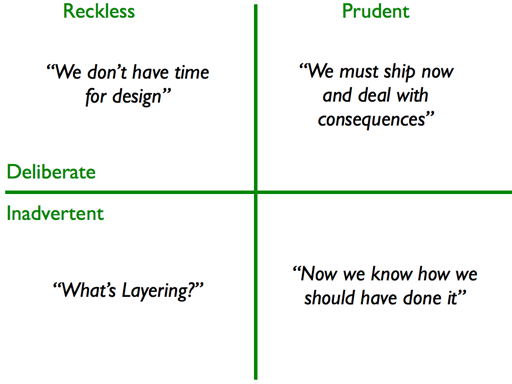
\includegraphics[width=.65\textwidth]{figures/literature_review/technical_debt_quadrant.png}
  \caption{Technical Debt Quadrant\cite{MartinFowler:TechnicalDebtQuadrant}}
  \label{fig:technical_debt_quadrant}
\end{figure*}
  
Figure \ref{fig:technical_debt_quadrant} presents the actual technical debt quadrant, and illustrates on each cell the possible cases that can happen with a development team while working on a software project. 

In addition, from the original description ``\textit{not quite right code which we postpone making it right}'' various people have used the metaphor of technical debt to describe many other \emph{kinds} of debts or faults of software development, including anything that is related to deploying, evolving a software system or anything that is intrinsic to software development such as test debt, people debt, architectural debt, requirement debt, documentation debt, or just an broad generalized software debt \cite{sterling2010book}. 

In this matter, Kruchten \textit{et al.}~\cite{kruchten2012IEEE} express their concern about how the use (or abuse) of the metaphor could spread it too thin making the metaphor lose its communication power. For example, a not yet implemented requirement, function, or feature does not translate to  requirement debt. Similarly, postponing the development of a new function is not a planning debt. Another danger pointed out by the authors relates to the assistance of static code analysis tools on the identification of technical debt. Although these tools are very useful there is a danger of equating whatever the tools can detect with what is technical debt. This approach leads to leaving aside large amounts of potential technical debt that is undetectable by tools, such as structural or architectural debt, technological gaps or self-admitted technical debt as discussed later on this chapter. 

Later, Spinola \textit{et al.} \cite{Spinola2013MTD} identified and organized a number of statements about technical debt expressed by practitioners in online websites, blogs and published papers. The authors chose 14 statements related to technical debt and conducted two surveys with 37 participants to evaluate the level of agreement on each statement. 
They found that practitioners strongly agree that if technical debt is not managed effectively, maintenance costs will increase at a rate that will eventually outrun the value it delivers to customers. In addition, they found that practitioners strongly disagree that all technical debt is intentional, the results found by the authors support the expanded technical debt definition proposed by McConnel and Fowler. 

Moreover, the authors state that the acceptance and use of the technical debt metaphor is in large part because it is easily understood. However, this can also be a concern to accurately define technical debt. Their reasoning is that because the technical debt metaphor is easy to understand, it is also easy to talk about, expand on, and relate experience to. A quick search of technical debt literature reveals subjective opinions, personal views, and catch phrases on such channels as blogs and online essays. Therefore, more analysis on the use of the metaphor is necessary to organize the technical debt landscape.

Alves \textit{et al.}~\cite{Alves2014MTD,Alves2016IST} proposes an ontology of terms on technical debt in order to organize a common vocabulary for the area. In their work they extracted and organized concepts derived from the results of a systematic literature mapping. In total, 100 studies, dated from 2010 to 2014, were evaluated. Their work contributed towards the evolution of the technical debt landscape through the organization of the different types of technical debt and their indicators. The authors found the following types of debt in the literature: design debt, architecture debt, documentation debt, test debt, code debt, defect debt, requirements debt, infrastructure debt, people debt, test automation debt, process debt, build debt, service debt, usability debt and versioning debt. Moreover, they state that some instances of technical debt can fit more than one type of technical debt. 

These works summarize the definition and expansion of the technical debt metaphor. 

\section{Identification and Implications of Technical Debt}

\subsection{Using Source Code and Static Analysis Tools}

A number of studies have focused on the detection and management of technical debt. Much of this work has been driven by the Managing Technical Debt Workshop community. Static analysis tools can help to detect source code anomalies and object oriented violations using metrics and thresholds to evaluate code quality. These violations are commonly referred as bad smells and they follow under the design technical debt type of debt. 

Zazworka \textit{et al.}~\cite{Zazworka2011MTD} conducted a case study to investigate how design debt, in the form of god classes, affects the maintainability of software projects. The authors analyzed two commercial applications of a small-size software development company. They found that god classes suffer more changes and contain more defects than non-god classes showing that technical debt has a negative impact on software quality, and should therefore be identified and managed closely in the development process.

Fontana \textit{et al.}~\cite{Fontana2012MTD} also analyzed design debt in the form of bas smells. The authors focus their attention on three specific code smells (i.e., god class, data class and duplicate code) extracted from open source systems of different domains. They proposed an approach to suggest which bad smell should be addressed first based on the negative impact they have on the quality of the project.

In a follow up study, Zazworka \textit{et al.}~\cite{Zazworka2013CSE} conducted an experiment where a development team was asked to identify technical debt items in artifacts from a software project that they were familiar with. Then, the authors collected the output of three static analysis tools to automatically identify technical debt and compared it to the results of human elicitation. The authors found that there is little overlap between the technical debt reported by different developers, so aggregation, rather than consensus, is an appropriate way to combine technical debt reported by multiple developers. Moreover, they confirmed that static analysis tools can not detect many different types of technical debt, and therefore, involving humans in the identification process is necessary. 

\subsection{Using Source Code Comments (Self-Admitted Technical Debt)}

A lot of effort has been made to identify and manage technical debt. Despite the help provided by static source code analysis tools the identification of technical debt is still an open challenge. More recently, Potdar and Shihab~\cite{Potdar2014ICSME} found that source code comments can be analyzed to identify technical debt. Differently from most source code analysis tools, that rely on suggested metrics and thresholds to detect a \emph{supposed} debt, technical debt found in the source comment is written by the developer of the program as a \emph{confession}. These developers are explicitly saying that a particular implementation is not ideal, in other words this implementation is \emph{self-admitted technical debt}. 

Potdar and Shihab~\cite{Potdar2014ICSME} conducted the first study to explore source code comments to identify technical debt. They extracted the source comments from 5 open source projects, and manually inspected them. In total, the authors read and analyzed more than 100K comments, and they come up with 62 different comment patterns that indicates the presence of \SATD. These comment patterns are words or small phrases such as ``retarded'', ``stupid'' and ``remove this ugly code''. Besides of the 62 comment patterns they found that \SATD comments are present in 2.4\% to 31\% of the analyzed files, that developers with higher experience tend to introduce most of the \SATD and that time pressures and complexity of the code do not correlate with the amount of self-admitted technical debt. This work is the current state-of-the-art in the identification of \SATD. 

Bavota and Russo~\cite{bavota2016MSR} presented differentiated replication of the work by Potdar and Shihab. The authors analyzed 159 software projects to investigate the diffusion and evolution of \SATD and its relationship with software quality. During this study the authors extracted over 600K commits and 2 Billion comments. Their main findings showed that \SATD is diffused, with an average of 51 instances per system, increases over time due to the introduction of new instances that are not fixed by developers, and even when fixed, it survives a long time (over 1,000 commits on average) in the system.

Also, Farias \textit{et al.}~\cite{Farias2015MTD} developed a Contextualized Vocabulary Model for identifying technical debt on code comments (CVM-TD). CVM-TD uses word classes and code tags to support technical debt identification based on the comment patterns devised in \cite{Potdar2014ICSME}. The model created by the authors provided a structure that systematically allows combining terms creating a large vocabulary on technical debt. However, the author point out that  CVM-TD needs to be calibrated in order to improve its accuracy. 

Wehaibi \textit{et al.}~\cite{wehaibi2016SANER} also took advantage of the comment patterns to examine the relation between \SATD and software quality. The authors analyzed if files with \SATD have more defects compared to files without \SATD, if \SATD changes are more likely to introduce future defects, and if \SATD changes tend to be more difficult. They analyzed 5 open source projects to find that there is no clear relationship between defects and \SATD, however, \SATD changes are more difficult to perform (i.e., they are more complex).

The work mentioned so far relied on the identification of technical debt through source code comments, specifically using the comment patterns approach. One aspect that is not explored however is how good is the comment patterns approach in identifying technical debt. Another topic that is not explored is that the comment patterns approach does not provide support for the identification of different types of technical debt. The first step to address the afore-mentioned limitations is to create a golden dataset of \SATD comments where different approaches can be compared in terms of precision and recall. Also, such dataset, if available could provide insights on the different types of \SATD. 

Believing that this is a very important step towards the advance of the state-of-the-art in the automatic identification of \SATD we focused our efforts to create an golden dataset of manually classified \SATD. In the next chapter we explain in detail our approach to create such a dataset of \SATD comments. We also analyze the insights achieved during the creation of this dataset, such as what are the different types of \SATD comments, how their distribution look likes and the definition of each type of \SATD.  